\documentclass[thesis.tex]{subfiles}

\begin{document}

\chapter{Prerequisites}\label{chap:preq}
In this chapter, the fundamentals necessary to understand the thesis will be explained in detail. Section~\ref{sec:sebasics} presents the basics of SE alongside its procedure and its types. Similarly, Section \ref{sec:spvsdp} elucidates the advantages and disadvantages of using 32-bit computations against 64-bit computations. Finally, the CUDA programming model is illustrated in Section \ref{sec:introcuda} along with a brief history and motivation.

\section{State Estimation}\label{sec:sebasics}
\subsection{Fundamentals}\label{subsec:fundamentals} 
Energy management is referred to as the continuous process of monitoring, coordinating and controlling of the generation, transmission and distribution of electricity in a power grid. The objectives of Energy Management Systems (EMS) are to minimize unforeseeable harm to the grid, implement safety regulations and supply power to the consumers with minimal disruptions.\\\\
Power grids are vast, complicated infrastructure systems and are comprised of busses that are geographically scattered. In order to safely monitor and administer a power grid, all the measurements from the grid must be centralized to a designated control center. These measurements are essential in functioning of the EMS. The system responsible for aggregation of these measurements is SCADA (Supervisory Control And Data Acquisition). \\\\
A SCADA system consists of the following:
\begin{enumerate}
	\item Remote Terminal Units (RTU): They are used to collect data from the remote locations.
	\item Communication Networks: They enable half-duplex communication among different devices.
	\item Master Terminal Unit (MTU): It ingests the information from the RTUs and generates information for display.
	\item Operator Console: This is the interface between the system and the operator.
\end{enumerate}
The on-site sensor readings acquired through RTUs are relayed across the communication networks in order to reach the MTU. These readings consist of active and reactive power injections, bus voltage RMS values and transmission line current. These measurements are susceptible to instrumentation and communication errors. Although great care is taken to guarantee accuracy, inevitable random noise is introduced in the measurements that can lead to distorted telemetered values. So as to generate a more realistic picture of the grid, these measurements are then fed to the State Estimation (SE) algorithm. The output of the process is a vector of voltage magnitudes and phase angles (i.e. state vector) which is then served as the input data to subsequent EMS applications as shown in Figure~\ref{fig:scada_to_SE_1}.\\\\
Scheweppe and his research group~\cite{Schweppe} introduced state estimation for electrical transmission grids in 1969 as a weighted-least-squares (WLS) problem that can be used to calculate state vector from all the busses in a given power grid at an arbitrary time. This is achieved by making several redundant network observations which yields an over-determined measurement dataset.
\begin{figure}[H]
	\centering
	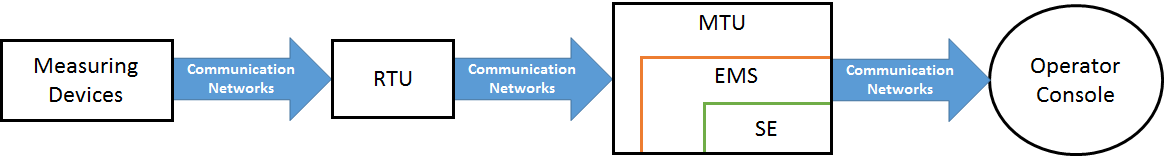
\includegraphics[scale=0.5]{scada_to_SE_1}
	\caption{Outline of data aggregation using SCADA for Power Grid Monitoring}
	\label{fig:scada_to_SE_1}
\end{figure}
Although SCADA is a mature and widely used technology, it suffers from a limitation where it cannot gather and transmit real-time measurements necessary for successful SE at all times. The unsynchronized data from SCADA systems is further accompanied by potential data loss and measurement errors originating from the sensors. To tackle this limitation, phasor measurement units (PMU) are introduced in the grid as shown in Figure~\ref{fig:scada_to_SE_2}. These devices are capable of obtaining synchronized measurements from an electrical grid using a common time source (e.g. GPS). These real-time observations when transmitted from many of different substations to the control room can be used for SE and acquiring a more accurate picture of the current state of the grid.
\begin{figure}[H]
	\centering
	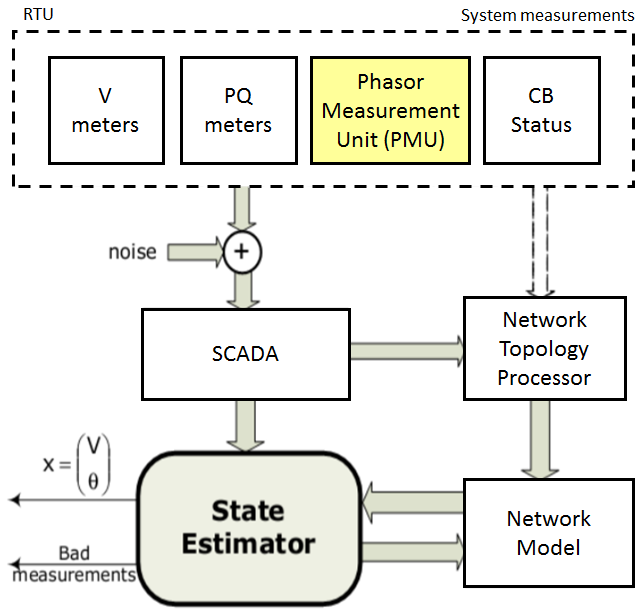
\includegraphics[scale=0.7]{scada_to_SE_2}
	\caption{State Estimation based on SCADA with PMU~\cite{Gaushell}}
	\label{fig:scada_to_SE_2}
\end{figure}
The obtained state vector from SE can be used for the purposes shown in the Figure~\ref{fig:uses_of_SE} below:
\begin{figure}[H]
	\centering
	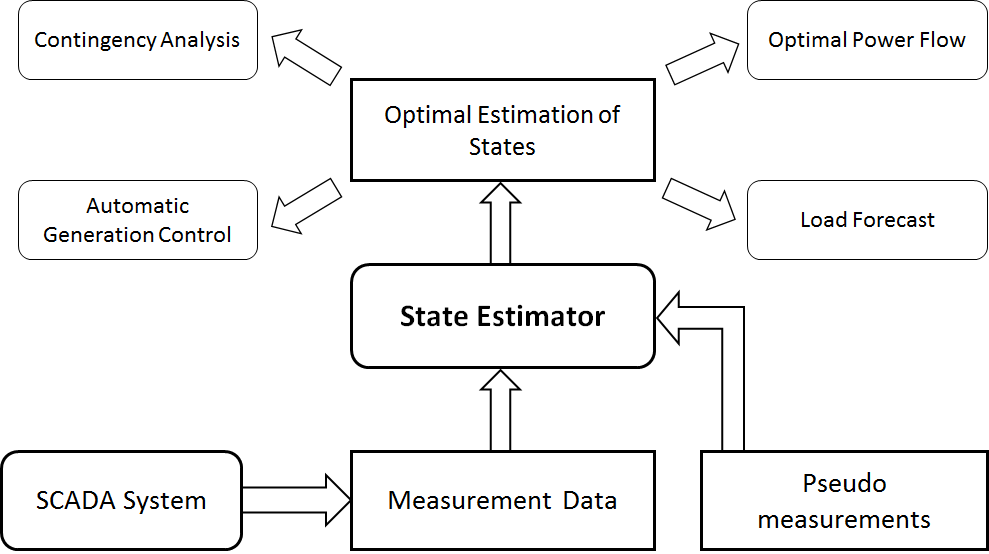
\includegraphics[scale=0.45]{uses_of_SE}
	\caption{Uses of State Estimation~\cite{Wilson}}
	\label{fig:uses_of_SE}
\end{figure}

\subsection{Method of State Estimation}
Although a broad class of techniques exist for SE, the most common and widely-accepted is the Weighted Least Squares (WLS) state estimator. This method makes certain prior assumptions about the raw measurements which are listed below~\cite{Wollenberg}:
\begin{enumerate}
	\item The expected value or average of the measurement noise is assumed to be zero. This means that the error within each measurement is equally probable to take a positive or negative value.
	\item The expected value of the square of the measurement error is Gaussian and the standard deviation of the same is \textbf{\textit{$\sigma$}}. Also, the measurements are independent of each other, i.e. the correlation between the measurements is zero. 
\end{enumerate}
As mentioned in Section~\ref{subsec:fundamentals}, the acquired measurements may be unreliable. Therefore, each measurement can be expressed along with an error component as follows:
\begin{equation}
\textbf{\textit{z}} = \textbf{\textit{z}}_{T} + \textbf{\textit{v}}
\end{equation}
where \textbf{\textit{z}} is the observed value, $\textbf{\textit{z}}_{T}$ is the true value and the measurement error is represented by $\textbf{\textit{v}}$. The relationship between the observed values and the real values can be expressed as follows:
\begin{equation}
\textbf{\textit{z}} = \textbf{\textit{h}}(\textbf{\textit{x}}) + \textbf{\textit{v}}
\end{equation}
where $\textbf{\textit{h(x)}}$ represents a vector of nonlinear functions. These functions associate the measured values \textbf{\textit{z}} to the state variables \textbf{\textit{x}}. 
With these noisy measurements, the states can be calculated by minimizing the performance index, \textbf{\textit{J}} (the weighted sum of square errors) expressed as follows:
\begin{equation}
\textbf{\textit{J}} = (\textbf{\textit{z}}-\textbf{\textit{h}}(\textbf{\textit{x}}))^{T}\textbf{\textit{R}}^{-1}(\textbf{\textit{z}}-\textbf{\textit{h}}(\textbf{\textit{x}}))
\end{equation}
where \textbf{\textit{R}} is the weighing factor. It is the diagonal covariance matrix of the measurements and can be expressed as follows:
\begin{equation}
\textbf{\textit{R}} = \begin{bmatrix}
{\sigma_{1}}^{2}& 0 & 0 & 0 & 0\\ 
0 & {\sigma_{2}}^{2} & 0 & 0 & 0\\ 
0 & 0 & ... & 0 & 0\\ 
0 & 0 & 0 & ... & 0\\ 
0 & 0 & 0 & 0 & {\sigma_{m}}^{2}
\end{bmatrix}
\end{equation}
The derivative of \textbf{\textit{J}} is taken to minimize the performance index \textbf{\textit{J}} and the following expression is obtained:
\begin{equation}\label{eq:dJ}
\textbf{\textit{g}}(\textbf{\textit{x}}^{k}) = \frac{\partial \textbf{\textit{J}}(\textbf{\textit{x}}))}{\partial \textbf{\textit{x}}} = -\textbf{\textit{H}}(\textbf{\textit{x}}^{k})\textbf{\textit{R}}^{-1}(\textbf{\textit{z}}-\textbf{\textit{h}}(\textbf{\textit{x}}^{k}))
\end{equation}
where $\textbf{\textit{x}}^{k}$ is the state vector at iteration $k$ and \textbf{\textit{H}} is the measurement Jacobian matrix defined as $\frac{\partial \textbf{\textit{h}}(\textbf{\textit{x}}))}{\partial \textbf{\textit{x}}}$.\\\\
Equation~\ref{eq:dJ}  can be used to obtain the Normal Equations by applying the Gauss-Newton method as follows:
\begin{equation}\label{eq:normaleq}
[\textbf{\textit{G}}(\textbf{\textit{x}}^{k})]\Delta \textbf{\textit{x}}^{(k+1)} = -\textbf{\textit{g}}(\textbf{\textit{x}}^{k})
\end{equation}
where \textbf{\textit{G}} is the gain matrix given by
\begin{equation}
\textbf{\textit{G}}(\textbf{\textit{x}}^{k}) = \frac{\partial \textbf{\textit{g}}(\textbf{\textit{x}}^{k})}{\partial \textbf{\textit{x}}} = \textbf{\textit{H}}(\textbf{\textit{x}}^{k})^{T} \textbf{\textit{R}}^{-1}\textbf{\textit{H}}(\textbf{\textit{x}}^{k})
\end{equation}
Hence, $\textbf{\textit{x}}$ is solved for iteratively till a convergence criterion of $\epsilon$ is met. Based on the above, the WLS SE algorithm can be presented as follows~\cite{Chen}:\\\\
\begin{algorithm}[H]
	\SetAlgoLined
	\KwData{Measurement matrix $\textbf{\textit{z}}$, Covariance matrix $\textbf{\textit{R}}$}
	\KwResult{State Vector $\textbf{\textit{x}}$}
	initialize $k = 0$\;
	initialize state vector $\textbf{\textit{x}}^k$ with a flat profile, e.g. $0\angle\ang{0}$\;
	 \While{$|\Delta \textbf{\textit{x}}^{k}| \geq \epsilon$} {
	 	Compute the measurement function: $\textbf{\textit{h}}(\textbf{\textit{x}}^{k})$\;
	 	Compute the measurement Jacobian: $\textbf{\textit{H}}(\textbf{\textit{x}}^{k})$\;
	 	Compute the gain matrix: $\textbf{\textit{G}}(\textbf{\textit{x}}^{k}) = \textbf{\textit{H}}^{T}(\textbf{\textit{x}}^{k})\textbf{\textit{R}}^{-1}\textbf{\textit{H}}(\textbf{\textit{x}}^{k})$\;
	 	 Compute the right-hand-side of the normal equation~\ref{eq:normaleq}: $-\textbf{\textit{H}}^{T}(\textbf{\textit{x}}^{k})\textbf{\textit{R}}^{-1}[\textbf{\textit{z}}-\textbf{\textit{h}}(\textbf{\textit{x}}^{k})]$\;
	 	 Solve Equation \ref{eq:normaleq} for $\Delta \textbf{\textit{x}}^{k}$\;
	 	 update $\textbf{\textit{x}}^{(k+1)} = \textbf{\textit{x}}^{k} + \Delta \textbf{\textit{x}}^{k}$\;
	 }
	\caption{Algorithm for State Estimation}
\end{algorithm}
\newpage 
\subsection{Comparison among Centralized, Parallelized \& Decentralized SE}
This section presents the comparisons among various approaches for state estimation in power grids based on the works of Richter et al~\cite{Richter2}\cite{Richter3}. The following Figure~\ref{fig:simple_SE} shows a simplified view of SE process:
\begin{figure}[H]
	\centering
	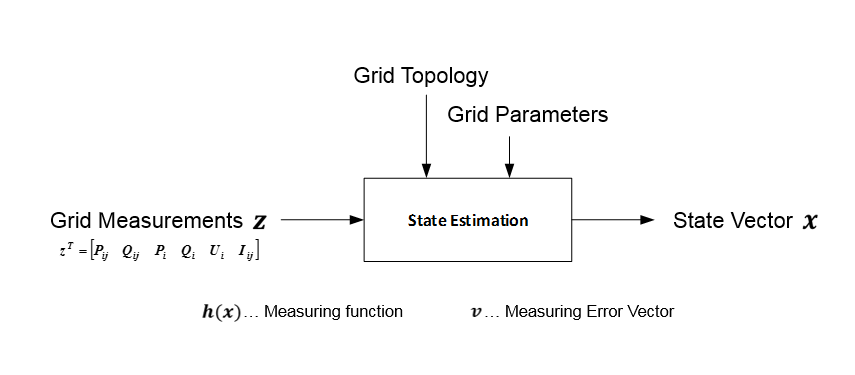
\includegraphics[scale=0.5]{simple_SE}
	\caption{Procedure of SE}
	\label{fig:simple_SE}
\end{figure}
\subsubsection{Centralized SE}
The type of SE discussed so far is centralized in nature. In general, the traditional centralized state estimator is situated inside a central control room as shown in Figure~\ref{fig:centralizedSE}. It gathers measurements from the power grid through the SCADA systems and computes the best estimate of the state. 
\begin{figure}[H]
	\centering
	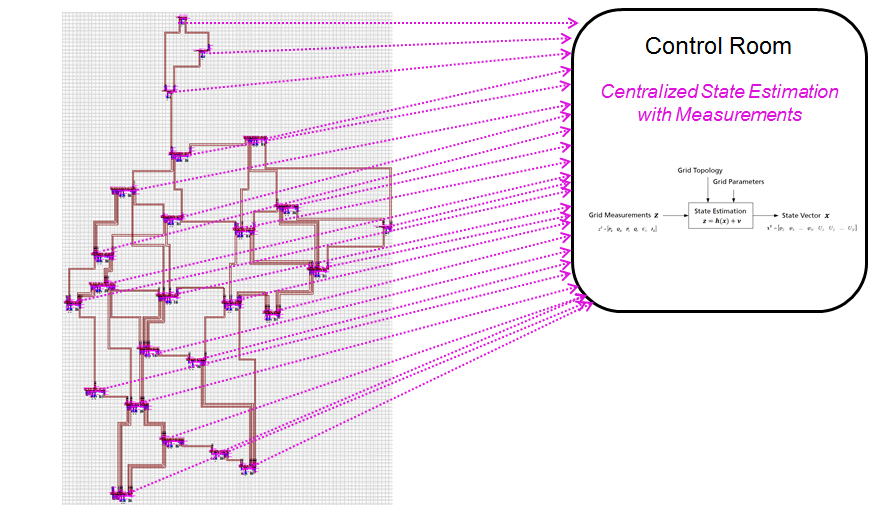
\includegraphics[scale=0.6]{centralizedSE}
	\caption{Centralized SE}
	\label{fig:centralizedSE}
\end{figure}
As seen in the Figure~\ref{fig:centralizedSE}, every station in the grid has direct communication with the control room. Such setup leads to the following issues:
\begin{enumerate}
	\item Large computational load.
	\item Larger computation load implies lower frequency with which SE can be performed.
	\item Large number of required communication channels for every station.
	\item Risk of synchronization errors.
\end{enumerate}
When the size of the power grid increases due to planned expansions, it escalates the aforementioned issues. A potential solution to handle the increased computational load could be the vertical scaling of the computing resources of the control room. However, despite dramatic rise in processing capacity in the past, progress of modern processors have stagnated~\cite{cpuStag}. More precisely, the effective compute power continues to grow but distributed across many cores. This stagnation in per-core processing throughput can slow down the desired frequency of SE in power grids. \\\\
Considering the above, there exists alternatives to centralized SE which reduce the computational burden by divide-and-conquer approach and are explained in the following subsections.

\subsubsection{Parallelized SE}
In parallelized SE, the control room splits the grid into logical sectors as illustrated in Figure~\ref{fig:parallelizedSE}. This may be done by studying the sparsity patterns of the Gain matrix $\textbf{\textit{G}}$~\cite{Abur}. The resultant smaller datasets lead to lower computational load. These datasets are then fed to a computer with dozens or hundreds of processing cores where the running state estimator can deploy each logical sector to a processing core with MIMD (multiple instruction, multiple data) processing capability~\cite{Abur}.
\begin{figure}[H]
	\centering
	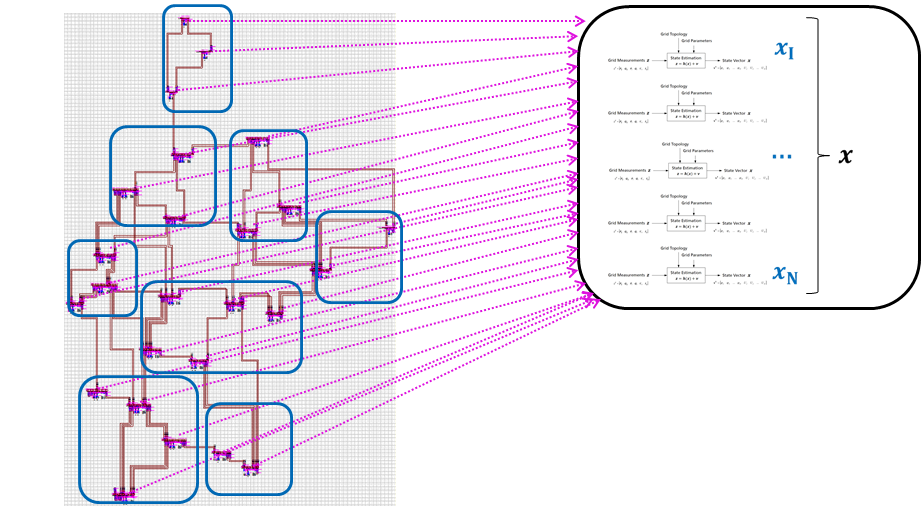
\includegraphics[scale=0.6]{parallelizedSE}
	\caption{Parallelized SE}
	\label{fig:parallelizedSE}
\end{figure}
This method is suitable for networks where synchronization is required among the processing-cores through interprocessor data communication. The synchronization usually occurs after every iteration of the WLS algorithm which may result in considerable processor idle times. On the other hand, if the parallel WLS is run in an asynchronous way, a drastic deterioration in the precision of SE vector is observed~\cite{Carvalho}.\\The advantages and disadvantages of this approach are as follows:\\
Advantages:
\begin{enumerate}
	\item Promising speedup ratios 
	\item Shared computational burden
\end{enumerate}

Disadvantage:
\begin{enumerate}
	\item Although the grid is sectorized, the centralized control center may still be the single point of failure.
	\item Large communication costs during data acquisition.
	\item Sizeable processor idle times due to per iteration synchronization barrier.
	\item Lower degree of observability per sector.
\end{enumerate}


\subsubsection{Decentralized SE}
This approach takes geographically distributed nature of power networks and increasingly sophisticated modern microprocessor-based RTUs  into consideration. These RTUs are capable of significant local processing before communicating to the control center~\cite{Carvalho}. Since the per-iteration synchronization barrier in parallelized SE is too costly if the processors are geographically far apart, decentralized SE offers an attractive alternative of asynchronous concurrent processing~\cite{Carvalho}.
\begin{figure}[H]
	\centering
	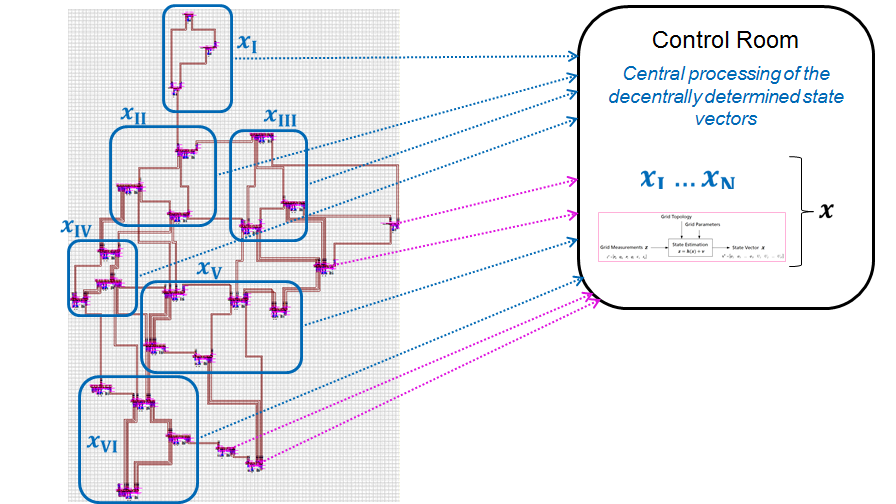
\includegraphics[scale=0.6]{decentralizedSE}
	\caption{Decentralized SE}
	\label{fig:decentralizedSE}
\end{figure}
In decentralized SE, the individual sectors preprocess the measurements $\textbf{\textit{z}}$ to find their respective state vectors as shown in Figure~\ref{fig:decentralizedSE}. Subsequently, the computed state vectors are communicated to the control room which then computes the global state vector.
The advantages and disadvantages of decentralized SE are as follows:\\
Advantages:
\begin{enumerate}
	\item Promising speedup ratios
	\item Shared computational burden
	\item No single point of failure
	\item Asynchronous concurrent execution
	\item Low data-transfer-related expenses
\end{enumerate}

Disadvantages:
\begin{enumerate}
	\item Potential loss of accuracy
	\item Presence of lone busses which cannot be assigned to any sector.
\end{enumerate}


\section{Single Precision vs. Double Precision }\label{sec:spvsdp}
Although converting decimal integers to binary format is relatively easy, expressing real numbers in machine-readable form is more difficult. In order to work approximately with real numbers (eg 1.3, Planck constant etc), computer systems provide floating point representations and related arithmetic support. During the initial years, several floating-point representations were proposed and used in earlier computers. However, since the varying representations hampered interoperability, since its introduction in 1985, the globally accepted floating-point representation is the IEEE 754 Standard~\cite{IEEE754}.\\\\
IEEE 754 Standard uses the idea of scientific notation to express real numbers in binary format and consists of a sign-bit, a mantissa and an exponent (with base 2).
\begin{figure}[H]
	\centering
	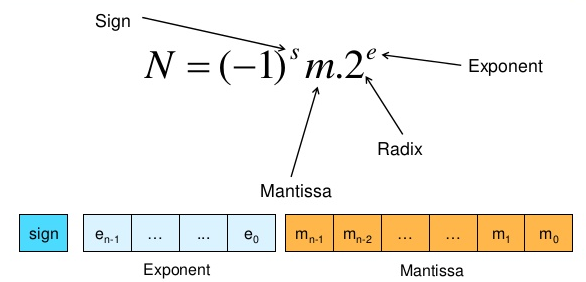
\includegraphics[scale=0.6]{FP}
	\caption{Representation of Floating Point Numbers}
	\label{fig:FP}
\end{figure}
Most scientific calculations need floating-point numbers. The speed of floating-point calculations is measured in FLOPS (floating-point operations per second). Most general purpose computers have one or more math coprocessors integrated within the CPU or as an add-on and they are specifically designed for carrying out floating point arithmetic operations. The most commonly used IEEE 754 representations are listed below:
\subsection{Single Precision Floating Point Numbers}
\begin{figure}[H]
	\centering
	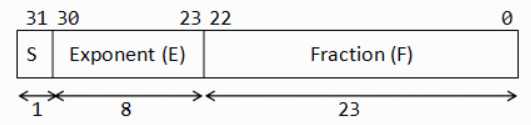
\includegraphics[scale=0.6]{FP32}
	\caption{Representation of 32-bit Single-Precision Floating Point Numbers}
	\label{fig:FP32}
\end{figure}
An IEEE 754 Single Precision floating-point number (a.k.a. FP32) occupies 32 bits in computer memory. It is known as float in Java, C/C++, C\# and Haskell, and as single in Visual Basic and MATLAB. Its accuracy can accommodate a decimal number with 7-8 digits.

\subsection{Double Precision Floating Point Numbers}
\begin{figure}[H]
	\centering
	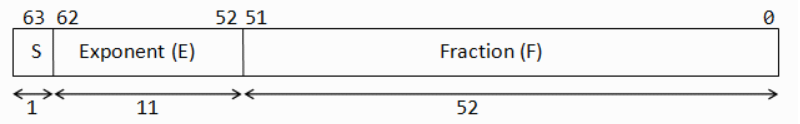
\includegraphics[scale=0.6]{FP64}
	\caption{Representation of 64-bit Double-Precision Floating Point Numbers}
	\label{fig:FP64}
\end{figure}
An IEEE 754 Double Precision floating-point number (a.k.a. FP64) occupies 64 bits in computer memory. It is known as double in Java, C/C++, C\# and MATLAB. Its accuracy can accommodate a decimal number with 15-16 digits.

\subsection{Issues and Limitations}
The limited number of bits available in both the precisions for real numbers enables only approximate representation. The approximation also gives rise to rounding and truncation errors for real numbers like 0.1. The amount of error introduced varies greatly depending on the precision used and gets propagated to other computations during program execution. Using Equation~\ref{roundingerrors}, we can see how the FP32 and FP64 summation errors varies programmtically for different values of $k$:
\begin{equation}\label{roundingerrors}
f(k)=\left | \frac{k}{10} - \sum_{i=1}^{k}0.1\right |
\end{equation}
Ideally, the value of $f(k)$ should be zero for every value of $k$. However, from Figure~\ref{fig:roundingError}, that proves to be untrue when tested on a computer. Hence, due to such rounding errors, programmers need to take great care in choosing appropriate precision for their applications and its criticality. 
\begin{figure}[H]
	\centering
	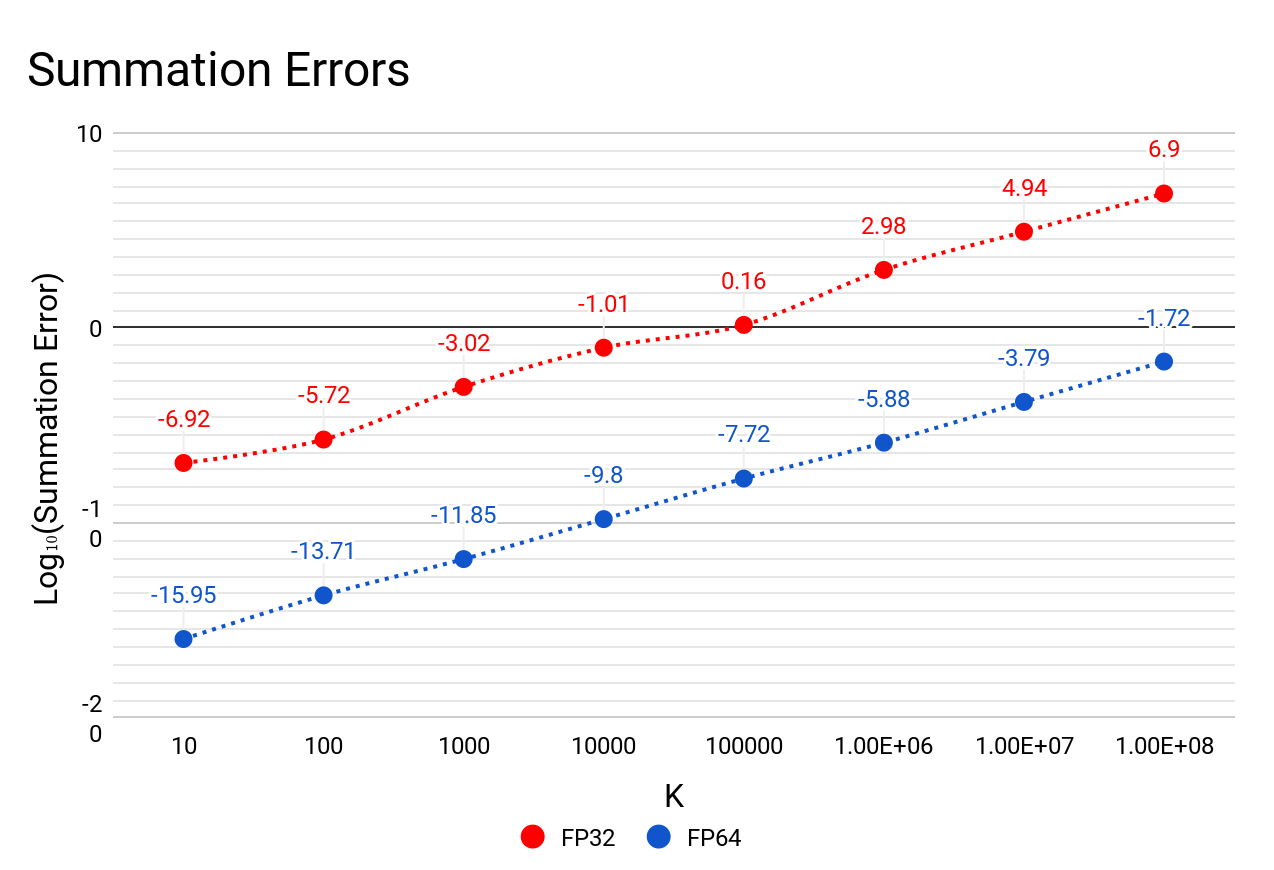
\includegraphics[scale=0.4]{roundingError}
	\caption{Rounding Errors using FP32 and FP64}
	\label{fig:roundingError}
\end{figure}


\section{Introduction to GPU and CUDA}\label{sec:introcuda}
Graphics Processing Units (GPUs) have covered a long way from functioning as a 
%mere single-core 
fixed-function hardware to a platform  for general-purpose high throughput computing using a large set of programmable cores. This section discusses the history of GPUs in computing alongside a review of the terminologies and the main features of NVIDIA’s GPGPU implementation. 
\subsection{History of GPU}
%The idea of specialized floating-point coprocessors that appeared attached to microprocessors (for running floating point instructions) in 1970s and 1980s inspired engineers to develop dedicated hardware support for displays. This became increasingly indispensable due to significant rise in use of graphics and PC games. This resulted with the release of ‘graphics card’ attached to CPU to generate video display. \\\\
By late 1990s, the computers needed support for 3D graphics, mainly because of use of graphics APIs such as DirectX and OpenGL in areas such as games. One of the important advancements before the development of GPU were programmable shaders which were effectively tiny programs that ran on the GPU to compute different effects and could apply the same operation to a large set of 3D points in a hugely parallel manner~\cite{ElsevierCUDA}. \\\\
The ‘world’s first GPU’ was released by NVIDIA in 1999 and was named GeForce 256. Advancements were made in GPU pipelines at the beginning of 21st century and these pipelines could be called for high-speed IEEE 754 floating point operations, in particular matrix and vector operations. In 2003, Mark Harris was among the first to recognize the potential of using graphical processing units (GPU) for general purpose applications which was followed by a push for general purpose GPU~\cite{Harris}.\\\\
In 2006, NVIDIA released the first GPU that could do general purpose computing as well as graphics processing and was based on Single-Instruction-Multiple-Thread (SIMT) architecture. This was followed by the release of CUDA (Compute Unified Device Architecture) which NVIDIA defines as ‘a parallel computing platform and programming model developed by NVIDIA for general computing on graphical processing units (GPUs)’~\cite{cuda}. CUDA enables the use of NVIDIA GPUs as coprocessors in order to accelerate certain parts of a program, generally those with a high computing load per data without having to learn sophisticated shader languages.

\subsection{Need for GPGPU}
Modern processors have reached a clock rate limit at around 4 GHz where the dissipated heat is high due to huge number of transistors and therefore special expensive cooling systems are required~\cite{ElsevierCUDA}.  For instance, Intel Core i7-8086K is estimated to have nearly 3 billion transistors with a base clock rate of 4.0 GHz and thermal design power (TDP) of 95W. The generational improvements in processor speeds at present have mostly stagnated and the processor manufacturers have permanently moved to a new paradigm: multicore processors. With this architectural shift from single-core design to modern multicore systems, the emphasis is now on parallelism in processing workloads and it can be of 3 fundamental types:
\begin{enumerate}
	\item Instruction-level Parallelism: The focus is on executing several instructions from the same instruction source across multiple cores.
	\item Task Parallelism: The focus is on distributing several independent functions from same application across multiple cores.
	\item Data Parallelism: The focus is on distributing several data items across multiple cores.
\end{enumerate}
Microprocessors are optimized for instruction-level and task-level parallelism. For arithmetic compute-intensive tasks which can be expressed as data-parallel operations, microprocessor’s sophisticated control logic and caching would be unnecessary. Fortunately, there exists are wide variety of arithmetic problems that can be expressed as such. Modern NVIDIA GPUs provide hundreds or thousands of simple compute cores (manycore design) that can be used for large data-parallel tasks with promising performance enhancement.\\\\
The figures~\ref{fig:throughputRise} and~\ref{fig:bandwidthRise} illustrate the change over past decade in floating-point capability between the CPU and the GPU. The observed discrepancy in floating-point capabilities is due to the fact that GPU design is based on SIMT architecture and is optimized for compute-intensive data-parallel tasks like graphics rendering. 
\begin{figure}[H]
	\centering
	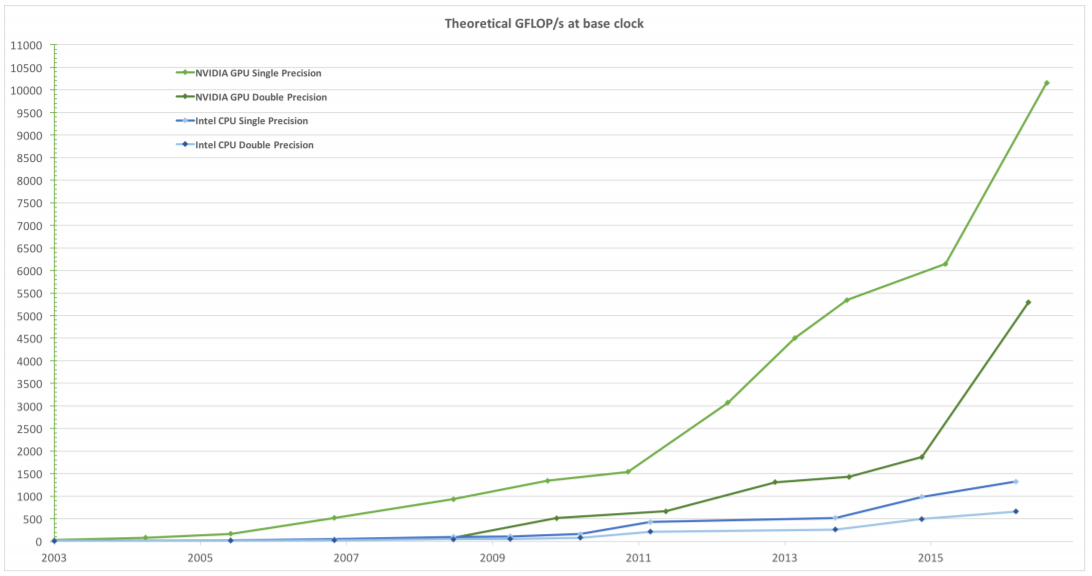
\includegraphics[scale=0.7]{throughputRise}
	\caption{Rise in Floating Point Arithmetic Throughput for CPU and GPU~\cite{cuda}}
	\label{fig:throughputRise}
\end{figure}
\begin{figure}[H]
	\centering
	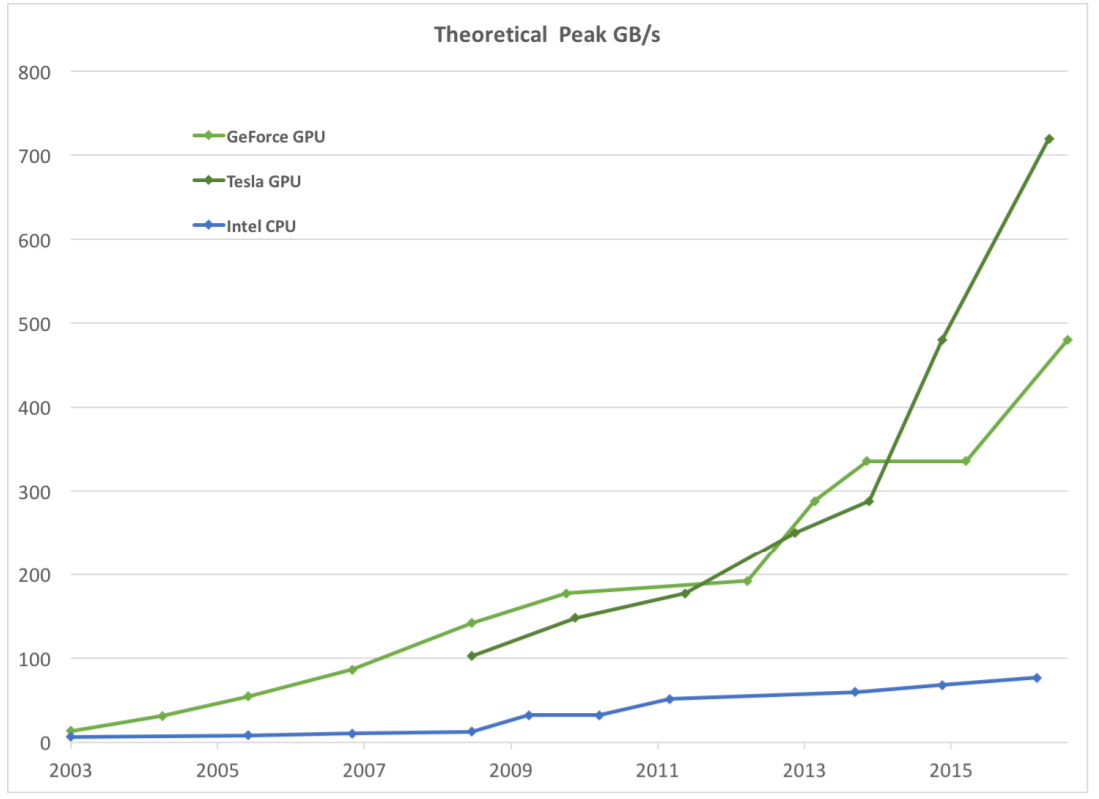
\includegraphics[scale=0.6]{bandwidthRise}
	\caption{Rise in Memory Bandwidth for CPU and GPU~\cite{cuda}}
	\label{fig:bandwidthRise}
\end{figure}
On the hardware level, GPUs have more transistors dedicated to data-processing instead of flow control or data caching. The differences in the schematics of a CPU and a GPU is illustrated below in Figure~\ref{fig:cpuvsgpuhardware}:
\begin{figure}[H]
	\centering
	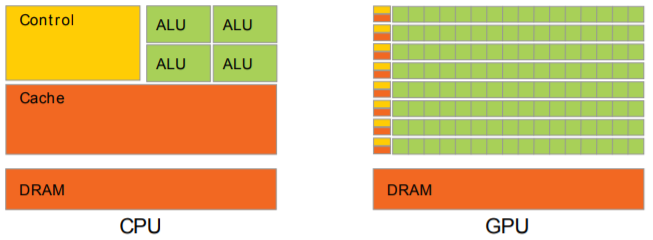
\includegraphics[scale=0.8]{cpuvsgpuhardware}
	\caption{GPU dedicates more transistors for data-processing~\cite{cuda}}
	\label{fig:cpuvsgpuhardware}
\end{figure}
If the problem at hand has a small data size and requires complex control logic with low-level parallelism, the CPU is a good choice since its optimized for handling unpredictable control flow and instruction-level-parallelism.  However, for workloads dealing with large amounts of data that can benefit from massive data parallelism and have high ratio of arithmetic operations to memory accesses, GPU is the right choice.
The table~\ref{tabular:UKJPNdata} below shows how a variety of applications from different domains have benefitted from the porting their problems to the GPU~\cite{cuda}.\\

{\renewcommand{\arraystretch}{1.1}%
\begin{table}[htp]
	\begin{tabular}{| *3{>{\centering\arraybackslash}m{1.9in}|} @{}m{0pt}@{}}
		\hline
		\textbf{Domain} & \textbf{Application} & \textbf{Speedup} &\\[2.1ex] 
		\hline
		Bioinformatics \& Life Sciences    & Sequencing and protein docking & 62x – 102x &\\[0ex]
		\hline
		Natural Disasters    & Tsunami Simulations & 60x &\\[0ex]
		\hline
		Machine Learning    & Speech/Multimedia Recognition & Up to 33x &\\[0ex]
		\hline
		Numerical Analytics    & $2^{nd}$ Order Wave Equation on MATLAB & 10x &\\[0ex]
		\hline
		Medical Imaging   & MRI Processing & 4x - 114x &\\[0ex]
		\hline
		Data Science \& Analytics   & Data Exploration Platform & 100x - 1000x &\\[0ex]
		\hline
	\end{tabular}
	\caption{Performance Boost using GPUs}
	\label{tabular:UKJPNdata}
\end{table}}


\subsection{Heterogeneous Computing}
Heterogeneous computing is referred to as use of a multicore microprocessor and one or more manycore GPUs as a coprocessor to the CPU. The GPUs are connected to the CPU via a PCI-Express. Since the GPU is effectively an add-on, it is referred to as the \textbf{device} whereas the CPU is called the \textbf{host}. 

CPU + GPU heterogeneous computing architectures deliver the best of both worlds by executing right workloads on the right components, i.e. by executing sequential or task-parallel sections on the host and the data-parallel computation-intensive sections on the device. \\
Hence, a heterogeneous application using GPUs consists of 2 parts:
\begin{itemize}
	\item Host code (control-intensive tasks)
	\item Device code (data-parallel computation-intensive tasks)
\end{itemize}
The  execution is started by the host and is responsible for managing the data, code and the runtime environment before issuing compute-intensive data-parallel tasks on the device. The host code is typically written in programming languages like C++, Java or FORTRAN whereas the device code in case of GPGPU is written using GPU computing frameworks like CUDA, OpenCL or HLSL. The following section introduces and describes CUDA in detail. 
\begin{figure}[H]
	\centering
	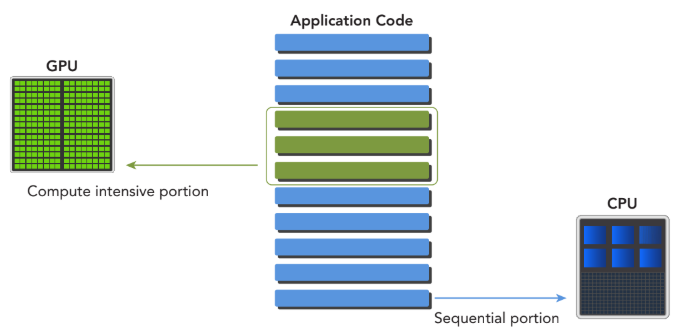
\includegraphics[scale=0.7]{loaddelegation}
	\caption{Assignment of workloads to suitable processors~\cite{profCUDA}}
	\label{fig:loaddelegation}
\end{figure}


\subsection{CUDA Programming Model}
CUDA is a general-purpose parallel computing platform and programming model that leverages the parallel compute engine in NVIDIA GPUs to solve many complex computational problems in a more efficient way while maintaining a low learning curve for programmers accustomed to popular programming languages like C.
CUDA consists of the following:
\begin{enumerate}
	\item Suitable NVIDIA GPU hardware along with its driver
	\item CUDA C compiler: \inlinecode{C}{nvcc}
	\item CUDA Runtime 
	\item Profiling Tools: \inlinecode{C}{nvprof}, NVIDIA Visual Profiler
\end{enumerate}
In addition to the above, CUDA provides the specification for the following on GPU:
\begin{enumerate}
	\item Programming model
	\item Execution model
	\item Memory model
\end{enumerate}
The programming, execution and memory models of CUDA are described in the following subsections.

\subsubsection{Programming Model: Kernels, Threads, Blocks \& Grids}
Kernels are important C language extension that enables programmers to define GPU functions in CUDA. A kernel is essentially a C function defined using \inlinecode{C}{\_\_global\_\_} declaration specifier and is executed N times in parallel by N different CUDA threads, unlike only once as typical C functions. These functions are launched from by the CPU. The number of threads that execute the launched kernel is specified using \inlinecode{C}{<<< . . . >>>} execution configuration syntax. \\
In the following sample code~\ref{code:elemArrAdd}, the kernel \inlinecode{C}{VecAdd} is launched on 1 block of N threads. Each thread that executes the kernel has a unique thread-ID which is 3-dimensional in nature. For this example, each thread with 1-D thread-ID ‘$n$’ would read from $n^{th}$ position of arrays \textbf{A} and \textbf{B} respectively, add them and store the result in nth position of array \textbf{C}. However, this would be occurring for all the threads executing in parallel.
\begin{lstlisting}[language=C, caption={Elementwise addition of two arrays A and B using CUDA}, captionpos=b, label={code:elemArrAdd}]
	// Device Code
	// Kernel definition
	__global__ void VecAdd(float* A, float* B, float* C)
	{
	int i = threadIdx.x;
	C[i] = A[i] + B[i];
	}
	
	// Host Code
	int main()
	{
	...
	// Kernel invocation with N threads
	VecAdd<<<1, N>>>(A, B, C);
	...
	}
	\caption{}
\end{lstlisting}
As shown in Figure~\ref{fig:cudathreadorganization}, the threads are organized in blocks. The blocks are three-dimensional in nature. Since all the threads in the same block get assigned to the same Streaming Multiprocessor(SM) and must share limited GPU resources, a block may contain only up to 1024 threads on current GPUs. The blocks can be further organized into one-dimensional, two-dimensional or three-dimensional grid of thread blocks and the upper limit on the number of blocks usually depends on the amount of data being processed or the number of SMs in the GPU.\\
Each thread knows its 3-dimensional block-local thread-ID and its block-ID. Combining both of them, each thread can calculate its global coordinates.
\begin{figure}[H]
	\centering
	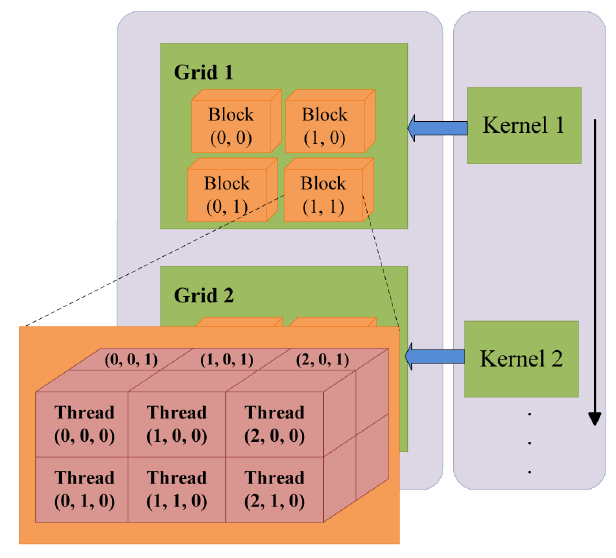
\includegraphics[scale=0.6]{cudathreadorganization}
	\caption{CUDA thread organization~\cite{cuda}}
	\label{fig:cudathreadorganization}
\end{figure}
From hardware perspective, the threads within a block are always executed simultaneously in groups of 32 where each group’s threads are processing the same instruction in SIMT fashion (NVIDIA’s SIMD architecture). It is the basic unit of execution in an SM and is referred to as a warp. The following Figure~\ref{fig:threadtowarps} illustrates the relationship between the logical view and the hardware view of a thread block.

\begin{figure}[H]
	\centering
	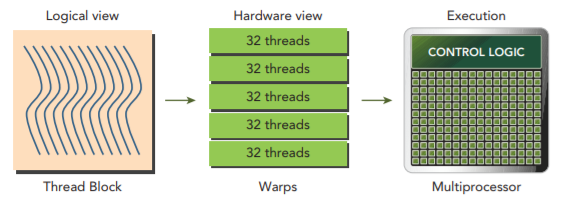
\includegraphics[scale=0.6]{threadtowarps}
	\caption{Grouping of CUDA threads from a block into warps~\cite{profCUDA}}
	\label{fig:threadtowarps}
\end{figure}


\subsubsection{Execution Model}
CUDA’s execution model can be enumerated as follows:
\begin{enumerate}
	\item A thread is mapped to a single computational core.
	\item A thread-block of threads is mapped to the same SM. It does not migrate to different SMs. 
	\begin{enumerate}
		\item Multiple concurrent blocks can be present on the same SM and depends on the resources available per SM.
		\item Threads in the same block can cooperate through shared-memory and synchronization barriers.
	\end{enumerate}
	\item A kernel which launches threads in thread-blocks to perform a compute-intensive operation gets mapped to the CUDA-enabled GPU and they may be launched concurrently or overlapped with data-transfers from the host via streams.
\end{enumerate}

\begin{figure}[H]
	\centering
	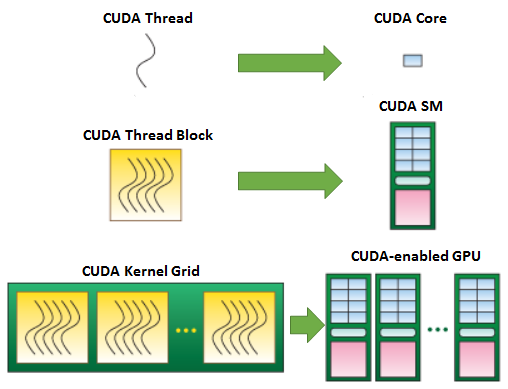
\includegraphics[scale=0.6]{cudaexecutionmodel}
	\caption{CUDA Execution Model}
	\label{fig:cudaexecutionmodel}
\end{figure}

According to NVIDIA, ‘CUDA architecture is constructed around a scalable array of Streaming Multiprocessors(SMs)’.  This is the reason behind transparent scalability of CUDA which enables the same CUDA program code to run on GPUs with different number of SMs in a way where a GPU with more multiprocessors will automatically execute the program in less time than a GPU with fewer multiprocessors. Figure~\ref{fig:smscalability} illustrates how CUDA manages necessary resource allocation across different GPUs.

\begin{figure}[H]
	\centering
	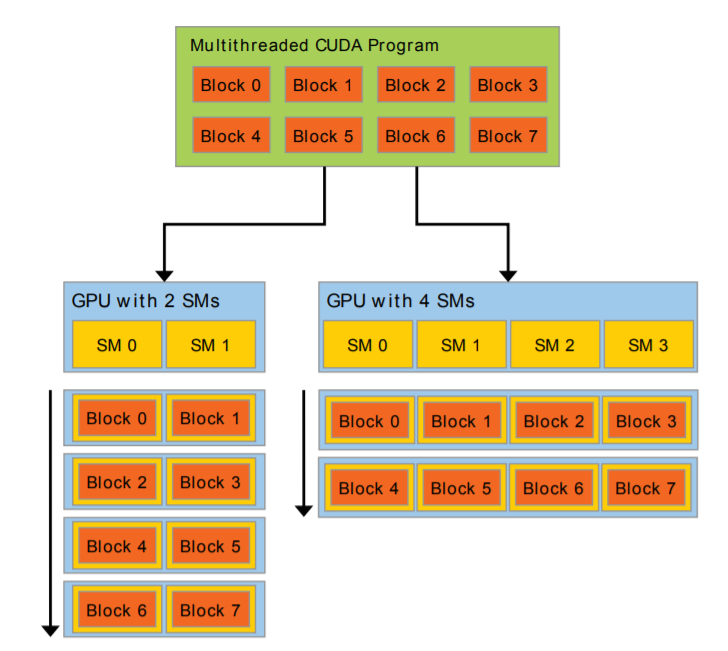
\includegraphics[scale=0.6]{smscalability}
	\caption{Transparent Scalability in CUDA~\cite{cuda}}
	\label{fig:smscalability}
\end{figure}

The programmers are required to partition the problem into coarse tasks which can be individually executed in parallel by blocks of threads. Each coarse task is further split into finer tasks that can be executed in parallel and in cooperation by the threads within the block. With this generalized approach of viewing the given problem at different granularities allows CUDA to transparently scale the program across GPUs with widely varying number of SMs. 

\subsubsection{Memory Model}
Apart from the non-programmable GPU caches (L1, L2, read-only constant \& read-only texture), CUDA memory model exposes the following types of programmable memories:
\begin{enumerate}
	\item Registers
	\begin{itemize}
		\item It is the fastest memory space onboard and is private to each thread. 
		\item Automatic variables declared within kernel are stored in registers.
		\item There is a hardware limit of 255 registers per thread.
	\end{itemize}
	\item Local Memory
	\begin{itemize}
		\item Variables in kernel that are too large to fit into registers are spilled into local memory.
		\item It is adjacent to global memory and is subject to requirement of coalesced memory accesses.
	\end{itemize}
	\item Shared Memory
	\begin{itemize}
		\item It is similar to CPU L1 cache and is also programmable.
		\item It is declared using \inlinecode{C}{\_\_shared\_\_} and delivers much higher bandwidth and lower latency relative to global or local memory.
		\item It is private to the each thread block and threads within the same block can share data in shared memory.
	\end{itemize}
	\item Global Memory
	\begin{itemize}
		\item It is the largest and most typically used memory on a GPU.
		\item Due to its high-latency, it is the slowest memory along with Constant and Texture memories unless its contents are cached.
		\item An allocation made on global memory exists throughout the lifetime of the application.
		\item Allocations can be made by the host using \inlinecode{C}{cudaMalloc} and it can be freed by using \inlinecode{C}{cudaFree}.
		\item It can be accessed via 32, 64 or 128 byte aligned memory transactions.
	\end{itemize}
	\item Constant Memory
	\begin{itemize}
		\item A constant memory variable can be declared using \inlinecode{C}{\_\_constant\_\_} keyword.
		\item Constant memory contents get cached dedicated per-SM constant cache.
		\item It is used to store values that would be later read by all threads in a warp, e.g. mathematical coefficients.
	\end{itemize}
	\item Texture Memory
	\begin{itemize}
		\item It is a type of global memory and is accessible through a per-SM dedicated read-only cache.
		\item The read-only cache supports hardware filtering  which can be used for performing floating-point interpolation as a part of the read process.
	\end{itemize}
\end{enumerate}
A typical CUDA application in general uses first 4 types of memory discussed. In conclusion, each thread in a kernel possesses its own private memory; a block of threads possesses its own shared memory and is destroyed when the block scopes out and a global memory that is accessible to all the threads and is retained throughout the lifetime of the application. Constant and Texture memories are read-only memories optimized for specialized purposes as described above. The following Figure~\ref{fig:cudamemorymodel} illustrates the CUDA memory hierarchy.

\begin{figure}[H]
	\centering
	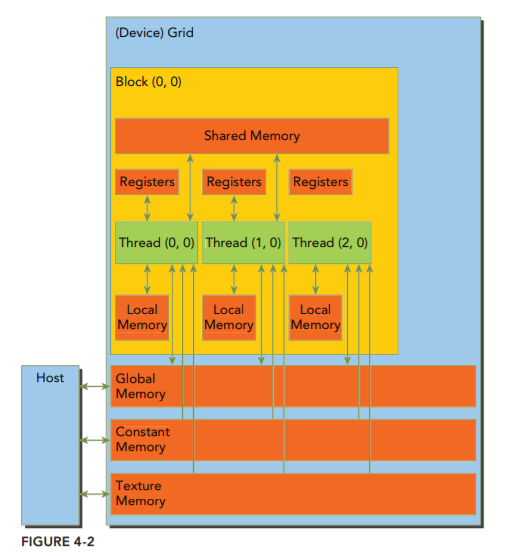
\includegraphics[scale=0.75]{cudamemorymodel}
	\caption{CUDA Memory Model~\cite{profCUDA}}
	\label{fig:cudamemorymodel}
\end{figure}

\subsubsection{CUDA in Practice}
\paragraph{Program Flow \& Device Concurrency:}
The typical flow of a heterogenous CUDA application can be generalized as below:
\begin{enumerate}
	\item Allocate pinned host memory and initialize it with problem datasets.
	\item Allocate device memory for the datasets
	\item Transfer contents of the host memory allocations to the device memory.
	\item Launch kernel(s) from the host. Kernel launches are asynchronous in nature.
	\item Transfer the results from the device memory to the host memory.
\end{enumerate}

This processing flow can be also extended to a multithreaded host application where each host thread can launch its own sequence of CUDA operations. This sequence of operations is executed in issue-order on the GPU and is referred to as a \textbf{CUDA stream}. Streams are particularly important because they can be used to execute operations concurrently on the hardware level. By creating separate streams for different threads, the sequence of CUDA operations can be mapped to different hardware work-queues of the GPU and much higher utilization can be achieved. NVIDIA GPUs equipped with Hyper-Q technologies provide 32 hardware work queues where operations without dependencies can be executed concurrently.\\
Figure~\ref{fig:serialstream} and~\ref{fig:parallelstreams} shows the execution of 8 kernels sequentially in the default stream and concurrently using individual stream per kernel launch respectively. 
\begin{figure}[H]
	\centering
	
\includegraphics[scale=0.75]{serialstream}
	\caption{Serialized kernel launch on the default stream}
	\label{fig:serialstream}
\end{figure}

\begin{figure}[H]
	\centering
	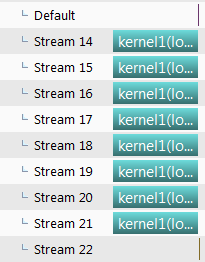
\includegraphics[scale=0.8]{parallelstreams}
	\caption{Concurrent kernel launches from multiple host threads}
	\label{fig:parallelstreams}
\end{figure}


\paragraph{CUDA Libraries:}CUDA platform offers several CUDA-accelerated libraries for industry standard programming languages such as C/C++, Fortran and Python. For most compute-intensive operations like linear algebra, FFT or learning of CNN, CUDA provides proprietary libraries which can be used out of the box. Some of these important libraries are:
\begin{itemize}
	\item For basic linear algebra, CUDA has its own BLAS implementation called cuBLAS.
	\item For solving linear systems, CUDA provides cuSOLVER library.
	\item For Fast Fourier Transforms, there is cuFFT library and so on.
\end{itemize}




\subfilebib % Makes bibliography available when compiling as subfile
\end{document}